\chapter{Paper I}\label{chap:paper1}
\section{Introduction}\label{sec:p1-intro}
In my first paper the aim is to establish the relationship between the efficiency of radial migration by cold torquing and the vertical action of stars. We seek to answer the question: do stars with large vertically extended obits migrate equally, or less efficiently, than those with smaller vertical extensions? Radial migration is a complicated process which can not be accurately described with an analytical expression. It is also a process which occurs over hundreds of millions of years, so we cannot observe it directly. For these reasons we make use of numerical or `$N$-body' simulations. In addition, using isolated disc galaxy simulations lets us have a great deal of control over the parameter space. 

The paper particularly focuses on determining the efficiency of radial migration as a function of the kinematics of their orbits. This is not a topic that has gone entirely without study, of course. The efficiency of radial migration as a function of radial velocity dispersion is investigated in \cite{solway:12}, \cite{vera-ciro:14}, and \cite{daniel:18} who all agree that migration is reduced with increased radial motion. A similar trend can be seen when investigating vertical motion or vertical scale height. This is studied by several articles including \cite{solway:12, vera-ciro:14, halle:2015, vera-ciro:16b} and the conclusion is the same: radial migration is reduced with increased vertical excursion measured either through scale height or velocity dispersion. This is dubbed the \textit{provenance bias} by \cite{vera-ciro:14}. However, \cite{solway:12} found that this effect was rather minor and was even used by \cite{schonrich:17} as justification for migration to be independent of actions in their model. They also speculate on the difference between the works of \cite{solway:12} and \cite{vera-ciro:14} being due to the strength and morphology of the spiral arms. 

The idea of a provenance bias can be understood by considering the interaction between a star and a spiral arm. Cold, circular orbits will spend more time near the corotation resonance of the spiral and be more prone to migration. However, a sufficiently strong spiral arm from a massive stellar disc, could perhaps be strong enough to migrate stars that reach larger vertical excursions as well. In \cite{vera-ciro:16b} they create three different simulations of live discs in static dark matter halo potentials. These go from a lighter disc to a heavier disc, with the heavier disc resulting in fewer, stronger, spirals \citep{donghia:15}. They claim that the provenance bias is present regardless of morphology which does not provide an explanation for the result of \cite{solway:12}.

In the paper we seek to answer how this provenance bias is affected by spiral morphology and disc dominance. To do this, we generate a large number of $N$-body simulations where the ratio of the halo to disc strength is varied to produce discs with different strength and morphology. We investigate the radial migration that occurs in these simulations and quantify it as a function of the disc dominance. Specifically we quantify the provenance bias of the migration. We determine that the slope of radial migration efficiency as a function of vertical action it itself a function of the dominance of the disc. The slope is steep for weaker discs (i.e., a provenance bias exists) and flattens for stronger discs, supporting the idea that strong spirals can migrate stars on vertically extended orbits. For radial action we find that there is a provenance bias regardless of disc dominance. 

\section{Setting up simulations}\label{sec:p1-simulations}
All of our simulations are setup and run using packages available as part of the \textsc{nemo}\footnote{\url{https://teuben.github.io/nemo/}}\citep{teuben:95} toolbox. We start with a pure $N$-body isolated galaxy system designed to be similar to the Milky Way. The scale lengths and masses of components we use are chosen with inspiration from \cite{mcmillan:17}. The full specifics of each component and the chosen parameters are found in paper I.

We follow the procedure of \cite{mcmillan:07} which describes the production of an equilibrium system of bulge, halo, and disc. The paper describes the procedure used in the \textsc{NEMO} package \textsc{mkgalaxy}, which in turn uses \textsc{mkwd99disc} and \textsc{mkhalo}. These are the packages we use to create our system as well. This disc has a standard shape with a density profile that decreases exponentially in radius and has a $\mathrm{sech}^2$ vertical profile:
\begin{equation}
    \rho_\mathrm{disc}(R, z) = \frac{1}{2z_\mathrm{d}} \Sigma_0 \exp\left(-\frac{R}{R_\mathrm{d}}\right) \mathrm{sech}^2\left(\frac{z}{z_\mathrm{d}}\right).
\end{equation}
The dark matter halo and bulge are both designed to have a spherical density distribution:
\begin{equation}
    \rho(r) = \frac{\rho_0}{x^\gamma_i(x^\eta + 1)^{(\gamma_o - \gamma_i)/\eta}} \mathrm{sech}\left(\frac{r}{r_t}\right),
\end{equation}
with the parameters chosen for the halo to provide a Dehnen-McLaughlin profile \citep{dehnen:05} which has the advantage of being fully analytic with a smooth transition between inner and outer parts of the distribution. It also matches very well to simulated dark matter halos. The bulge uses a standard Hernquist profile \citep{hernquist:90}.

Starting from these initial conditions we change only the mass of the dark matter halo. We create eleven different setups with halo masses ranging from $1.7\times 10^{11}\ \mathrm{M}_\odot$ to $1.02\times 10^{12}\ \mathrm{M}_\odot$ which corresponds to the ratio of the radial force from the halo to the disc, $F_\mathrm{h}/F_\mathrm{d}$, ranging from around 0.5 to 3.2 at $R = 8$ kpc and $z = 0$. In other words, we go from disc-dominated systems to halo-dominated systems. Each dark matter halo setup is also generated with ten different random seeds to estimate stochasticity, resulting in a total of 110 simulations.

\section{Evolution of non-axisymmetric features}\label{sec:p1-evolution}
\begin{figure}[t]
    \centering
    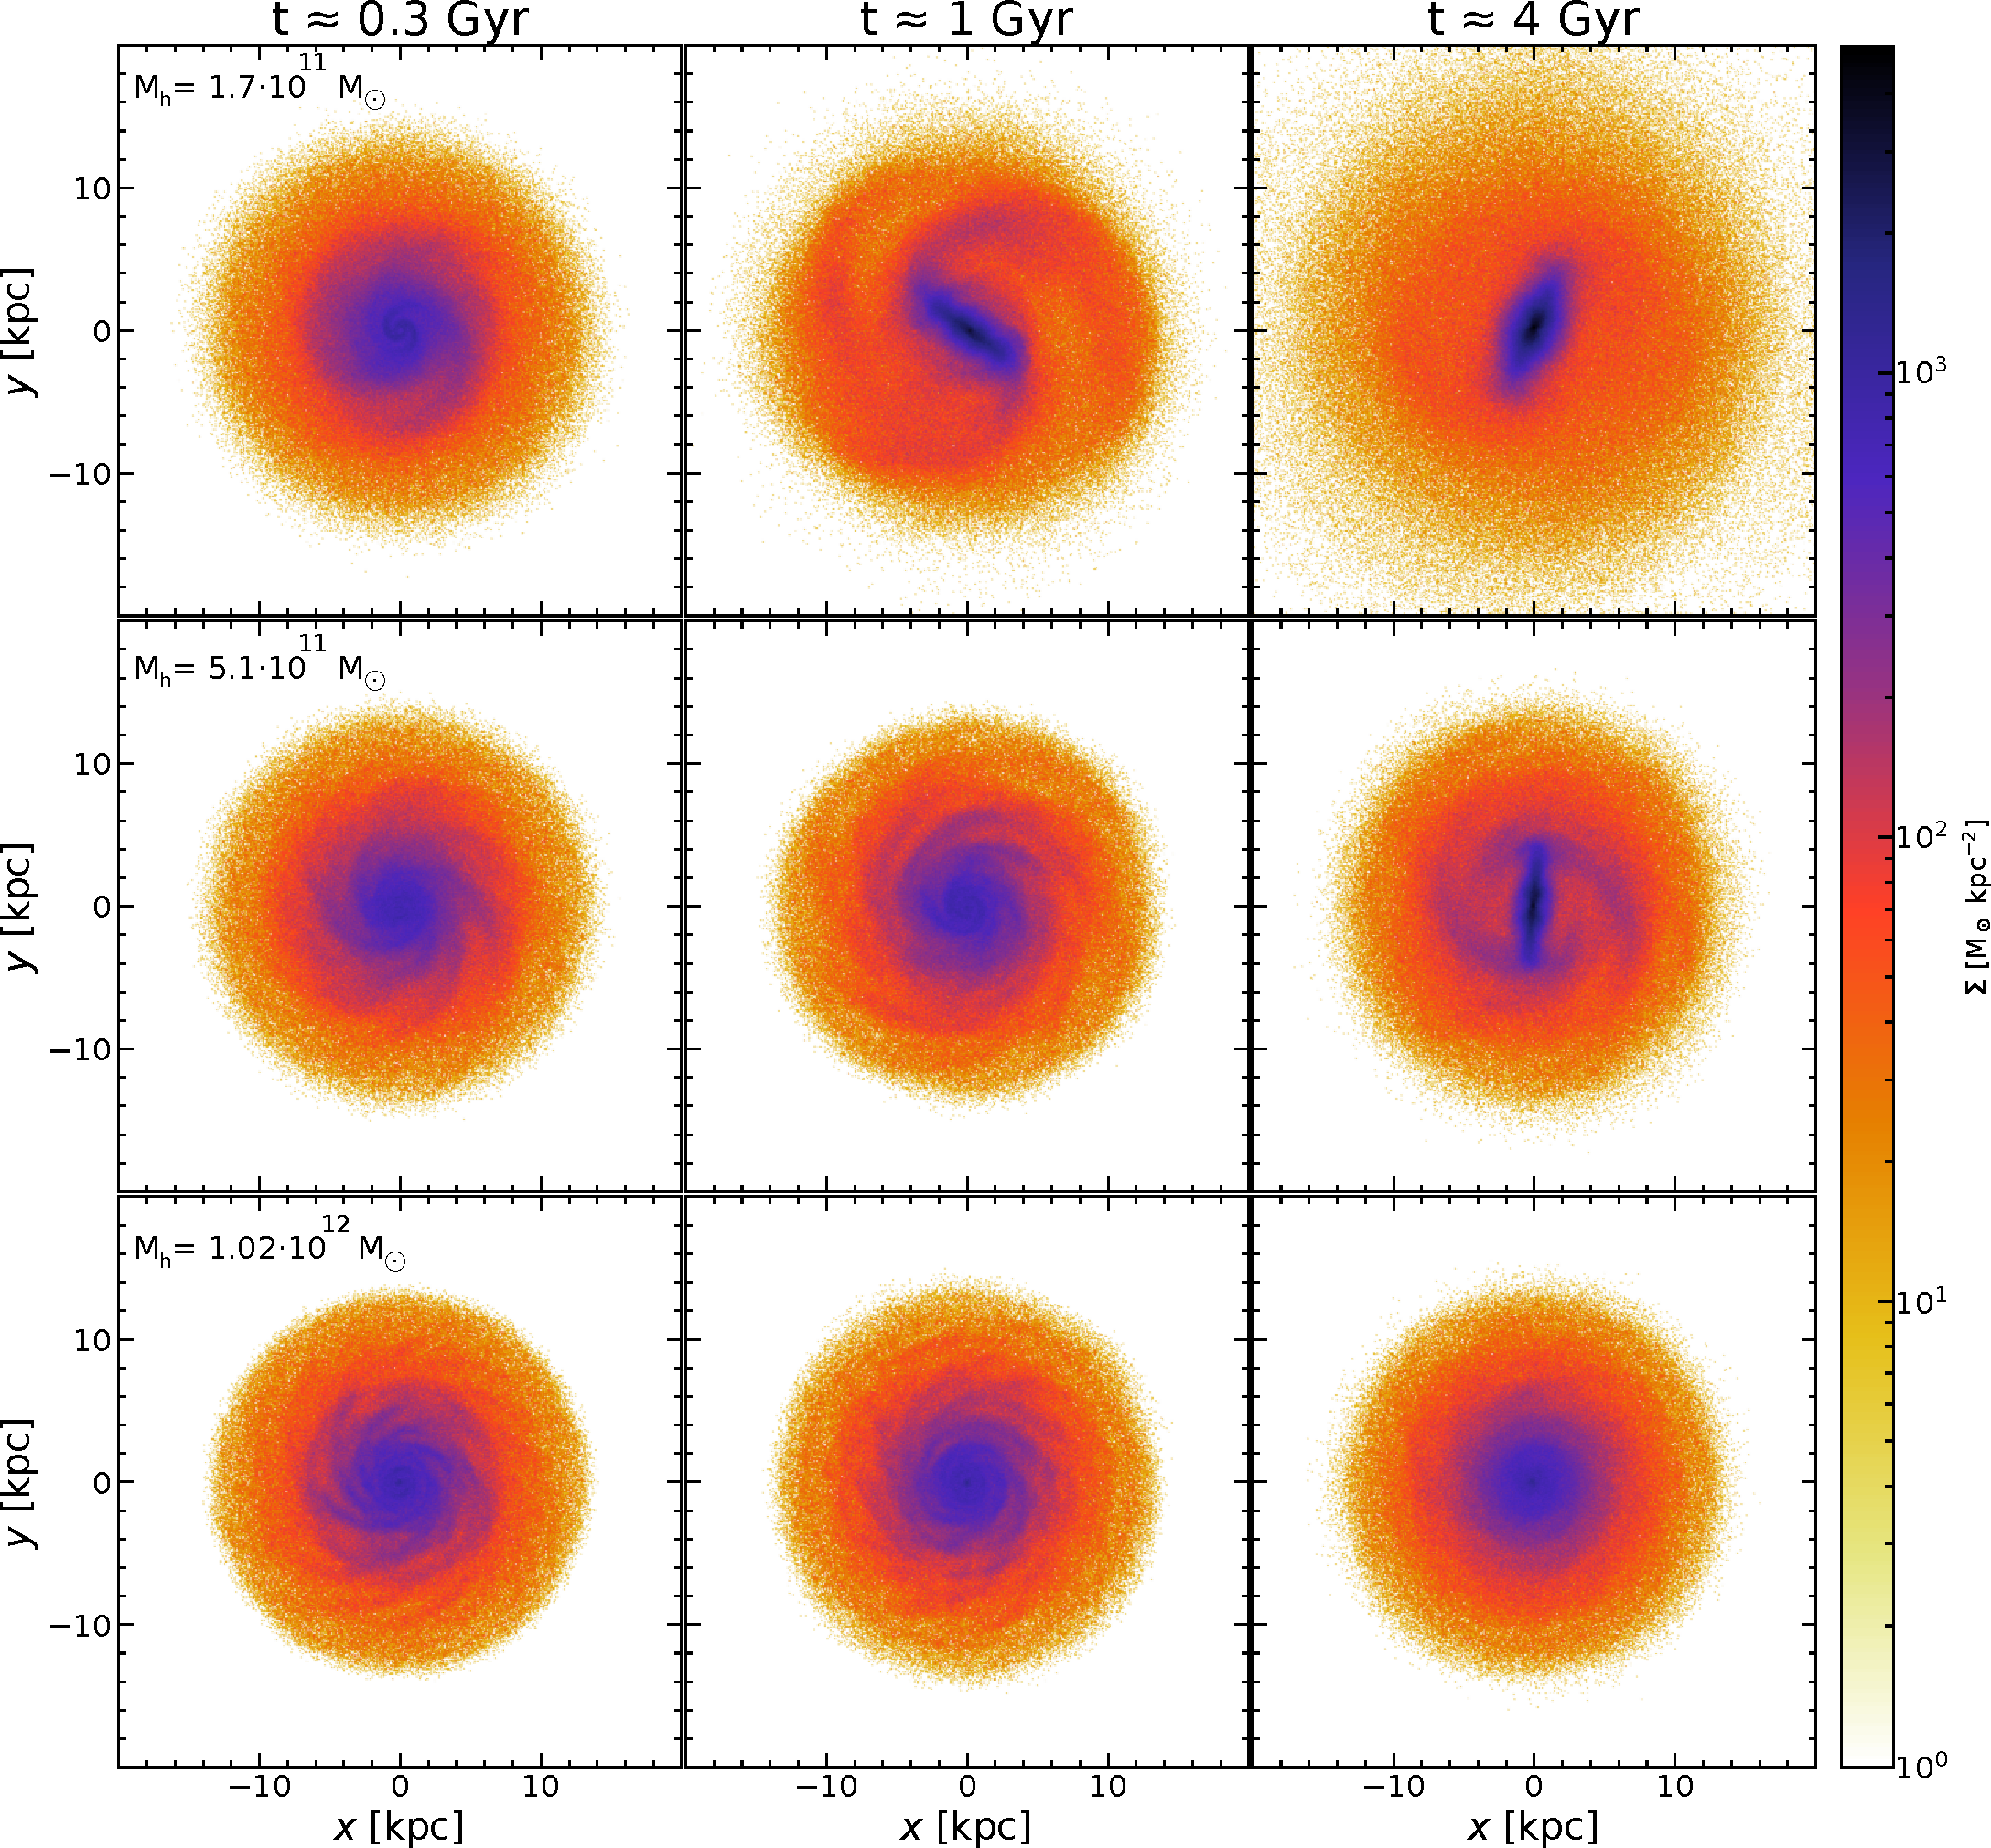
\includegraphics[width=0.9\textwidth]{images/evolution.pdf}
    \caption{Three simulated galaxies seen face-on with masses: $1.02\times 10^{12}\ \mathrm{M}_\odot$,  $5.1\times 10^{11}\ \mathrm{M}_\odot$, $1.02\times 10^{12}\ \mathrm{M}_\odot$ in each row. The time of the snapshots for each column is indicated on the top. The different evolution of non-axisymmetric features is seen.} % Fig. 2.1
    \label{fig:evolution}
\end{figure}
To capture the evolution of the simulated galaxies and their spiral arms and bars we use two approaches. The first is a direct visual inspection of the disc morphology in the plane of rotation at three different times, which correspond to `early', `evolved', and `late' times or 0.3 Gyr, 1 Gyr, and 4 Gyr respectively. This is shown in Fig. \ref{fig:evolution}. Since we are in a pure $N$-body simulation, we do not get much secular evolution beyond this time as the disk kinematics become too heated to participate in the dynamical interactions with the spiral arms. For this analysis we also only look at the lightest halo, $1.7\times 10^{11}\ \mathrm{M}_\odot$; the heaviest halo, $1.02\times 10^{12}\ \mathrm{M}_\odot$; and the one in between, $5.1\times 10^{11}\ \mathrm{M}_\odot$ as representative cases. This gives a disc-dominated case, a halo dominated case, and something in between. 

These simulations highlight that a very halo-dominated system leads to many, weaker arms rather than grand-design spirals and is unable to form a bar as well. In contrast to this, the disc-dominated system shows impressive arms, a bar, as well as the heating mentioned before as the disc becomes extended by comparison to its quiescent counterparts.

The second approach is using a Fourier analysis to extract the power spectrum of different modes, $m$, or number of spiral arms ($m=2$ is atwo-armed spiral or bar). This method is described thoroughly in \cite{roskar:12} and in our paper. This analysis further strengthens what is already discussed above. The disc-dominated system sees a strong $m=2$ resonance arise already at around 0.3 Gyr, probably a mixture between the spirals and bar. It has a pattern speed of ${\sim}30$ km s$^{-1}$ kpc$^{-1}$, comparable to that of the Milky Way bar. The intermediate disc takes until after 2 Gyr to form a $m=2$ feature with weaker multi-arm features prior to this time. Finally the halo-dominated system barely sees any significant modes appear apart from a very weak $m=6$ feature briefly around 0.2 Gyr. Our results agree with \cite{donghia:15} that the disc-dominated systems form fewer, stronger spirals. This, of course, has implications for the radial migration.

\section{Quantifying radial migration}\label{sec:p1-quantifying}
\begin{figure}[t]
    \centering
    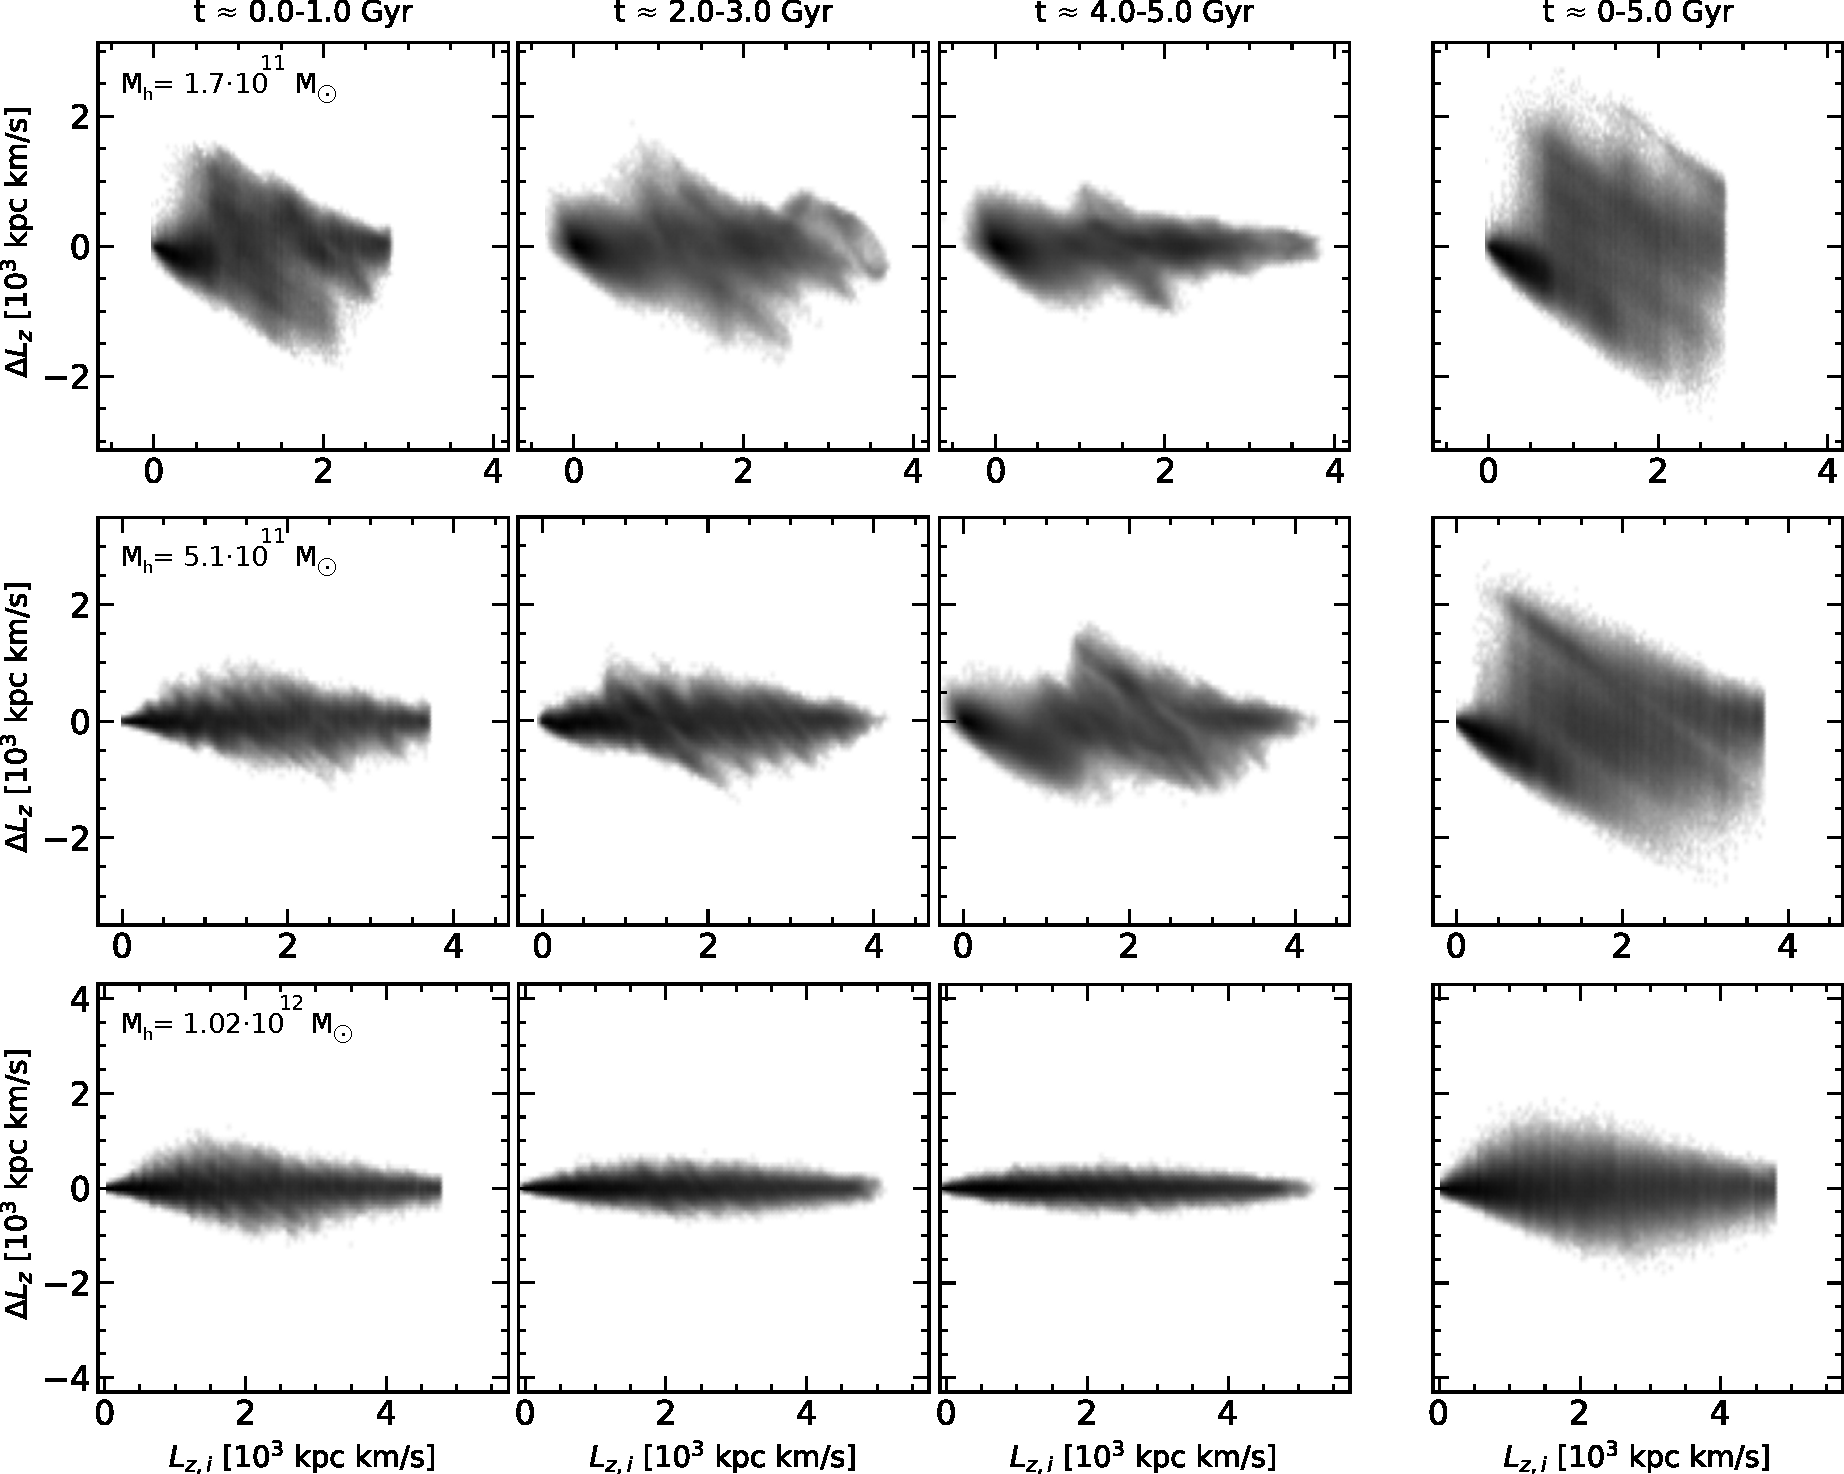
\includegraphics[width=1\textwidth]{images/dlz.pdf}
    \caption{Change in angular momentum, $\Delta L_z$, between two points in time as a function of initial angular momentum, $L_{z, \mathrm{i}}$. The rows correspond to the same simulations as in Fig. \ref{fig:evolution} and the time of angular momentum change is shown at the top. The amount of angular momentum change in each case is closely related to the evolution of strong non-axisymmetric features in the simulation.} % Fig. 2.2
    \label{fig:dlz}
\end{figure}
\begin{figure}[t]
    \centering
    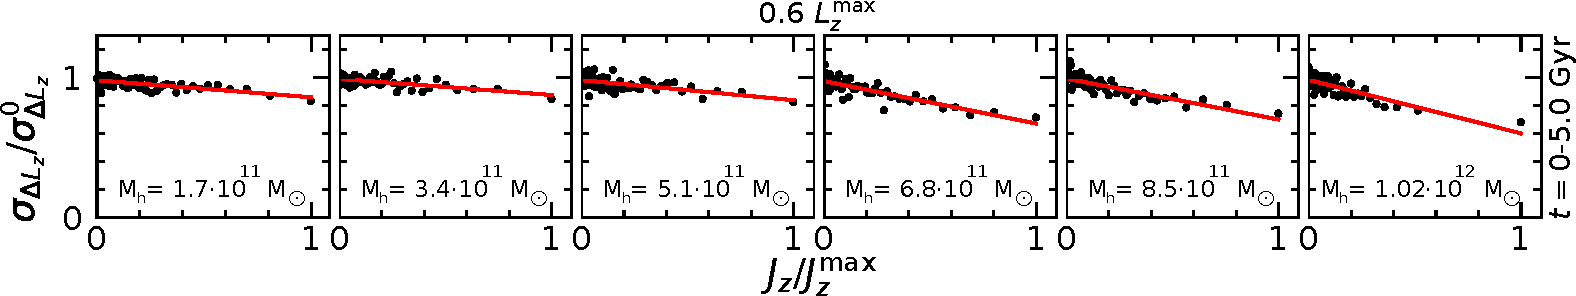
\includegraphics[width=1\textwidth]{images/slopes.pdf}
    \caption{Change in angular momentum, $\Delta L_z$, between two points in time as a function of initial angular momentum, $L_{z, \mathrm{i}}$. The rows correspond to the same simulations as in Fig. \ref{fig:evolution} and the time of angular momentum change is shown at the top. The amount of angular momentum change in each case is closely related to the evolution of strong non-axisymmetric features in the simulation.} % Fig. 2.3
    \label{fig:slopes}
\end{figure}
To gauge the amount of radial migration that occurs across the disc, we use a common approach of looking at the change in angular momentum, $\Delta L_z = L_z(t_2) - L_z(t_1)$, between two points in time $t_1$ and $t_2$. This can be compared against the initial angular momentum of the particles, $L_{z, \mathrm{i}}$, which is a proxy for the guiding radius. This is seen in \ref{fig:dlz} for the three simulations mentioned in section \ref{sec:p1-evolution} and shows how the strength of the secular features affects the migration. Note that diagonal features in this space corresponds to migration across a corotation resonance since particles interior to the resonance are migrated outwards, gaining a positive $\Delta L_z$ and vice-versa for the particles exterior. For example, consider the intermediate case. As was shown in the previous section, the bar forms not until after 2 Gyrs to form its largest $m=2$ mode. We can see here that the most significant migration does not transpire until after this. We also see that the disc-dominated system has strong early migration which calms down as the disc has become heated. Since we have quantified the amount of migration as a function of angular momentum and shown that how it relates to the disc morphology, we are equipped to tackle the primary question, the provenance bias.

We want to see how the migration changes as a function of the vertical action $J_z$ across the disc. The particles are therefore binned 100x100 in the space of initial vertical action, $J_{z, \mathrm{i}}$, and initial angular momentum, $L_{z, \mathrm{i}}$. In each of these bins, the amount of migration occurring is quantified by the dispersion of angular momentum changes, $\sigma_{\Delta L_z}$, which we call the radial migration \textit{efficiency}. We can then separate different bins in $L_{z, \mathrm{i}}$ into separate cases and investigate the behaviour of migration efficiency $\sigma_{\Delta L_z}$ as a function of initial vertical action $J_{z, \mathrm{i}}$. In the paper we use three values of $L_{z, \mathrm{i}}$ as representative of separate radial disc regions: 0.4, 0.6, and 0.8 of the maximum $L_{z, \mathrm{i}}$, corresponding to about 15 kpc. In this overview, we will show the $0.6 L_z^\mathrm{max}$ case only. There are also inconsistencies between the simulations and in radius that require special attention. At smaller guiding radius particles reach much larger extents in vertical action due to the gravitational potential. To correct for this $J_z$ is normalized such that it ranges from 0 to 1 with 1 corresponding to the largest extent in $J_z$. We also know that total migration is less in the halo-dominated simulations (as seen in Fig. \ref{fig:dlz}). We wish to know how migration is biased to higher vertical actions, rather than how much migration occurs in total, and so we also normalize $\sigma_{\Delta L_z}$ by dividing it by the its value at $J_z = 0$ km s$^{-1}$ kpc$^{-1}$. The result as seen in Fig. \ref{fig:slopes} allows us to determine the slope in this space, which is a measure of the provenance bias. A flat slope means that migration is equally efficient at all values of $J_z$ and a strong negative slope means that migration preferentially affects low $J_z$ particles.

This result shows that the provenance bias is a function of the disc dominance of the simulated system. We see the same trend in the slopes at the two other angular momentum slices considered, $0.4 L_z^\mathrm{max}$ and $0.8 L_z^\mathrm{max}$. We compare our results with \cite{vera-ciro:16b} by reproducing their Milky-Way like simulation and altering the disc dominance through the disc mass. We then apply our analysis approach to these simulations and quantify the migration in the same way as for our own simulations. This leads us to the same conclusion as above: the slope of migration efficiency flattens with disc dominance. The fact that we see this and they do not is likely because of the lengths we go to in order to quantify the migration. We also investigate the radial bias of migration efficiency to find that there is a provenance bias that is independent of disc dominance, suggesting different responses to cold torquing efficiency with increased action in the disc plane instead of orthogonal to it.

These results have significant implications for galaxy evolution. If stars on vertically extended orbits, which are typically older, can be migrated then any interpretation of stellar distributions as a function of age are contaminated. The results also provide necessary constraints for analytical modeling of radial migration, which is a necessary part of any analytical galaxy evolution model.
